% ****** Start of file apssamp.tex ******
%
%   This file is part of the APS files in the REVTeX 4.1 distribution.
%   Version 4.1r of REVTeX, August 2010
%
%   Copyright (c) 2009, 2010 The American Physical Society.
%
%   See the REVTeX 4 README file for restrictions and more information.
%
% TeX'ing this file requires that you have AMS-LaTeX 2.0 installed
% as well as the rest of the prerequisites for REVTeX 4.1
%
% See the REVTeX 4 README file
% It also requires running BibTeX. The commands are as follows:
%
%  1)  latex apssamp.tex
%  2)  bibtex apssamp
%  3)  latex apssamp.tex
%  4)  latex apssamp.tex
%
\documentclass[%
 reprint,
%superscriptaddress,
%groupedaddress,
%unsortedaddress,
%runinaddress,
%frontmatterverbose, 
%preprint,
%showpacs,preprintnumbers,
%nofootinbib,
%nobibnotes,
%bibnotes,
 amsmath,amssymb,
 aps,
%pra,
%prb,
%rmp,
%prstab,
%prstper,
%floatfix,
]{revtex4-1}

\usepackage{graphicx}% Include figure files
\usepackage{dcolumn}% Align table columns on decimal point
\usepackage{bm}% bold math
%\usepackage{hyperref}% add hypertext capabilities
%\usepackage[mathlines]{lineno}% Enable numbering of text and display math
%\linenumbers\relax % Commence numbering lines

%\usepackage[showframe,%Uncomment any one of the following lines to test 
%%scale=0.7, marginratio={1:1, 2:3}, ignoreall,% default settings
%%text={7in,10in},centering,
%%margin=1.5in,
%%total={6.5in,8.75in}, top=1.2in, left=0.9in, includefoot,
%%height=10in,a5paper,hmargin={3cm,0.8in},
%]{geometry}

%%%%%%%%%%%%%%%%%%%%%%%%%%%%%%%%%%%%%%%%%%%%%%%%%%%%%%%%%%%%%%%%%%%%%
%  needed macros:

%text macros:

\def\etal{{\it et al.}}
\def\etc{{\it etc.}}
\def\eg{{\it e.g.}}

% math mode macros:

\def\ee{e^+e^-} 

%%%%%%%%%%%%%%%%%%%%%%%%%%%%%%%%%%%%%%%%%%%%%%%%%%%%%%%%%%%%%%%%%%%%%%


\begin{document}

\preprint{LCCPEB---}

\title{The International Linear Collider \\ A Global Project}% Force line breaks with \\
\thanks{Version 1.3}%

\author{Jim Brau}
% \altaffiliation[Also at ]{Physics Department, XYZ University.}%Lines break automatically or can be forced with \\
\author{etal}%
 \email{Second.Author@institution.edu}
\affiliation{%
 Authors' institution and/or address\\
% This line break forced with \textbackslash\textbackslash
}%

\collaboration{Linear Collider Collaboration}%\noaffiliation

\date{\today}% It is always \today, today,
             %  but any date may be explicitly specified

\begin{abstract}
Input from the International Linear Collider community for the European Strategy Update 

\end{abstract}

\pacs{Valid PACS appear here}% PACS, the Physics and Astronomy
                             % Classification Scheme.
%\keywords{Suggested keywords}%Use showkeys class option if keyword
                              %display desired
\maketitle

%\tableofcontents

\section{\label{sec:intro}Introduction}

1 page - Jim and Juan

    Introduce the ILC250, brief overview of status (technical maturity and TDR, staging, cost analysis, status of political situation)


\section{\label{sec:phys}Physics}

[2 pages - Michael, Christophe, Keisuke, Jenny, Junping]

The physics case for the construction of the ILC is very strong.   The
most important item in this case is the ability to study the couplings
of the Higgs boson with high precision.  The ILC at 250~GeV also
presents many opportunities to discover new particles that go beyond
the capabilities of the LHC.  Finally, the ILC at 250~GeV opens the
door to further exploration of $\ee$ reactions at higher energies. 
The ILC physics case is reviewed at greater length in the reference
document~\cite{ILCforESS}. 

The Higgs boson is a necessary yet also mysterious part of the
Standard Model of Particle Physics (SM).    In the SM, the Higgs field
couples to every elementary particle and provides the mass for all
quarks, leptons, and heavy vector bosons.   The LHC has now discovered
the Higgs particle and confirmed the couplings responsible for the
masses of the $W$, $Z$, $t$, $b$, and $\tau$ at the qualitative
level~\cite{LHCHiggssummary}.  However, many mysteries could still be
buried here.   The Higgs couplings are not universal, as the gauge
couplings are, and their pattern (which is also the pattern of lepton
and quark masses) is not explained by the SM.  The basic phenomenon that provides
mass for elementary particles---the spontaneous breaking of the gauge
symmetry $SU(2)\times U(1)$---is not explained, and actually cannot be
explained, by the SM.   The Higgs boson could also couple to new
particles and fields that have no SM gauge interactions and are
otherwise completely inaccessible to observation.  Thus, detailed
examination of the Higgs boson properties should be the next major
goal for particle physics experiements.

Within the SM, the couplings of the Higgs boson are specified now that
the parameters of the model, including the Higgs boson mass, are
known.  Expected improvements in the SM parameters in the 2020's will
allow these couplings to be predicted to the part-per-mille level~\cite{Lepage:2014fla}.
Models of new physics correct  these predictions.   These corrections
are predicted to be small, at the 10\% level or below, but they can
be visible to precision experiments.   Most importantly, different
classes of models affect the various Higgs couplings differently, so that
systematic measurement of the Higgs couplings can reveal clues to the
nature of the new intereractions.   The precision study of the Higgs
boson interactions then provides a new method both to {\it discover}  the
presence of physics beyond the SM and to {\it learn}  about its nature.

The couplings of the Higgs boson are now being studied at the LHC, but
it is unlikely that the LHC experiments will be able to reach the
level of precision required for sensitivity to new physics models. 
It is important to remember that the goal of
precision Higgs measurement is not to confirm the SM at a given level
of accuracy but rather to discover robust deviations from the SM
pattern that are signals of new physics.   For all Higgs decay modes in which the
Higgs boson does not appear as a resonance (that is, for all decays
except those to 
$\gamma\gamma$ and $4\ell$), Higgs boson event samples at the LHC are dominated
by SM background processes.  Complex selections are needed to make the
Higgs boson component visible. A few percent modelling uncertainty in
the estimation of the SM backgrounds
 destroys the ability to measure Higgs couplings at the 5\%
level.  Further, since this uncertainty is a systematic error, it will
always leave the question of whether deviations from the SM have truly
been observed.

What is needed for a precision Higgs boson measurement program
is a new experimental method in which all individual Higgs boson decay events
are manifest
and can be studied in detail.   This is provided by the reaction
$\ee\to Zh$ at 250~GeV in the center of mass.
  With small and precisely calculable SM backgrounds, any $Z$ boson
  observed with a lab energy of 110~GeV is recoiling against a Higgs
  boson.   Selecting such events gives the profile of Higgs boson
  decays, in SM leptonic and hadron modes and even in invisible or
  partially visible exotic modes. 

Further, since the cross section for Higgs production can be measured
without measuring any property of the Higgs boson, the scale of Higgs
couplings can be determined and the individual couplings can be
absolutely normalized.  Each individual coupling can be compared to
its SM prediction.

In the description of new physics by an  $SU(2)\times U(1)$-invariant
effective field theory (EFT), new physics effects on the  Higgs boson
couplings to $W$ and $Z$ are related to new physics effects on
precision electroweak observables and in $\ee\to W^+W^-$.   This
latter reaction can also be studied to high precision at an $\ee$
collider.  Beam polarization at the ILC is at especially powerful tool
to separate the contributions of different EFT
coefficients.    In \cite{Barklow:2017suo}, it is shown that {\it all}
relevant EFT
coefficients can be fit {\it simultaneously} from the multiple
observables available at the ILC, giving a 
determination of Higgs boson couplings that is as
model-independent as the EFT description itself. 
 This analysis is reviewed in detail in
\cite{ILCforESS}. 
For the nominal ILC program at 250~GeV, we predict that the Higgs
coupling to $b$ quarks will be measured to 1\% accuracy and the
couplings to $W$ and $Z$ to 0.7\% accuracy.  The spectrum of  expected
measurements is shown in Fig.~\ref{fig:Higgssummary}.  Note that the 
discovery of any anomaly at 250~GeV can be confirmed in running at
500~GeV 
using additional reactions  such as $WW$ fusion production of the
Higgs boson.   Measurements at this
level can discover---and distinguish---models of new physics over a
wide space of possibilities, even for models in which the predicted new
particles are too heavy to be discovered at the LHC~\cite{Barklow:2017suo}.

%%%%%%%%%%%%%%%%
\begin{figure}
\begin{center}
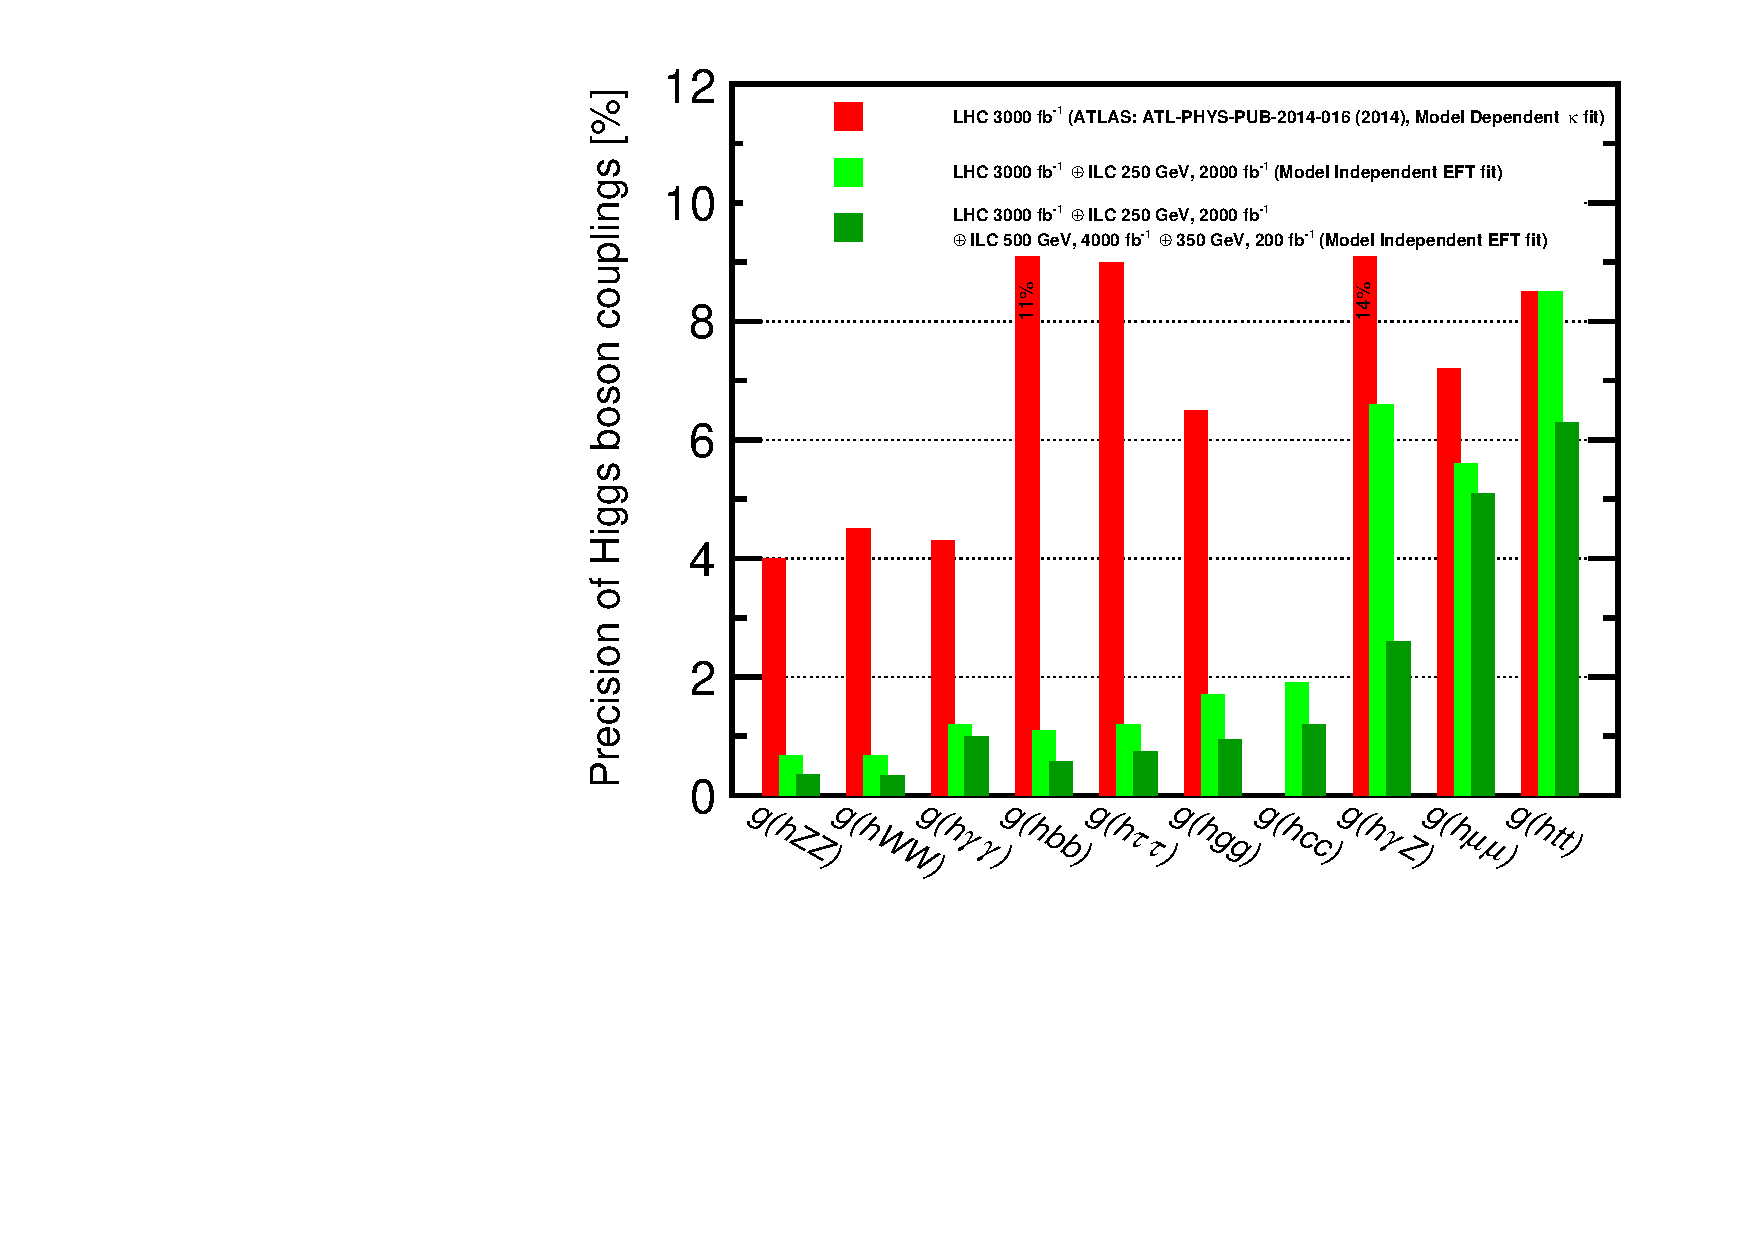
\includegraphics[width=0.95\hsize]{figures/DeltaH_EFT.pdf}
\end{center}
\caption{Projected Higgs boson coupling uncertainties for the ILC
  program at 250~GeV and an energy upgrade to 500~GeV, from \cite{Fujii:2017vwa}, 
 These projections are compared to
  the results of model-dependent estimates for HL-LHC uncertainties 
presented by the ATLAS 
collaboration~\cite{H2aaLHC}. [Note: the LHC projections will be
updated in the fall of 2018.]}
\label{fig:Higgssummary}
\end{figure}
%%%%%%%%%%%%%%%%%%%%%%%%%%%%%%%%%%%%%%%%%%%%%%%%%%%%%%%%%%%%%%

In addition to decays predicted in the SM, the Higgs boson could decay
to particles with no SM gauge interactions.    These decays may
include invisible decays (\eg, to a pair of dark matter particles $\chi$)  or
partially invisible decays (\eg, to $b\bar b \chi \chi$).   The ILC
can robustly seach for all types of exotic decays  to the part per
mille level of branching ratios~\cite{Liu:2016zki}.

The ILC can also search for particles produced through electroweak
interactions, closing gaps that are left by searches at the LHC.  An
important example is the Higgsino of supersymmetric models.   If the
mass  differences among Higgsinos is smaller than a few GeV---which is
actually the prediction of currently allowed models---then Higgsinos
of 100~GeV mass would be produced copiously at the LHC, but this
production would not be registered by LHC triggers.  In the clean
environment 
of the ILC, even such fragile signatures as this 
would be discovered and the new particles 
studied with percent-level precision~\cite{Higgsino}.

 ILC precision
measurements of $\ee\to f\bar f$ processes at 250~GeV have a sensitivity to new
electroweak gauge bosons comparable to (and complementary with) 
direct searches at the LHC.  The reaction $\ee\to b\bar b$ is
particularly interesting, since models of the top quark mass with
composite Higgs bosons can give significant corrections in this
reaction~\cite{eetobb}.

The ILC at 250~GeV can be the first step to the study of $\ee$
reactions at higher energy.   A linear $\ee$ collider is extendable in
energy by making the accelerator longer or by improving the
acceleration gradient. Extensions to 500~GeV and 1~TeV were envisioned
in ILC Technical Design Report~\cite{Behnke:2013xla}.    These would offer a
measurement of the top quark mass to 40~MeV, measurements of the top
quark electroweak couplings to the per-mille level, measurement of the
Higgs coupling to the top quark to 2\% accuracy, and measurement of
the triple Higgs boson coupling to 10\%  accuracy. They  also would be
the setting for much 
deeper searches for new particles with electroweak interactions.
A higher-gradient accelerator in the ILC tunnel could reach even
higher energies.  The
ILC promises a long future beyond its initial 250~GeV stage.




\section{\label{sec:collider}Collider}

2 pages - Benno, Shin

    Summary of the ILC250 design (important to note the elements that are retained in first stage to accommodate future energy extensions)

\section{\label{sec:detect}Detectors and R\&D}

2 pages - Ties, Andy


The science at the ILC drives the requirements on detectors. The main factors are:
\begin{itemize}
 \item The detector has to have an excellent track momentum
   resolution. The benchmark reaction here is the analysis 
of the di-lepton mass in the process $HZ \to H \ell^+
\ell^-$. This reaction allows the reconstruction of the 
Higgs mass independent of its decay mode via the 
reconstruction of the lepton recoil spectrum. In order that 
the momentum resolution of the detector does not limit 
the mass resolution achievable for the recoiling lepton 
system, stringent momentum resolution requirements have to be met. 
\item The reconstruction of the flavour of the final state can 
often be done best with the help of lifetime information of the 
decaying particles. For this, very powerful vertex detectors 
are needed. This is particularly important 
in the Higgs sector, where -- at least for light Higgs bosons -- 
a large fraction of the Higgs decays has bottom 
quarks in the final state. Many other physics signatures will 
produce complex final states with bottom or charm quarks as well. 
A supreme vertex detector therefore is needed to reconstruct these 
long lived particles with excellent resolution. 
\item The overall event is best reconstructed with the 
particle flow measurement. The particle flow technique combines 
the information from the tracking systems and from the 
calorimetric systems in an attempt to reconstruct the 
energy and the direction of all charged and 
neutral particles in the event. To minimize overlaps between 
neighboring particles, and to maximize the probability to 
correctly combine tracking and calorimeter information, 
excellent calorimeters are needed with very high granularity. 
\item Many physics signatures predict some undetectable particles, 
which escape from the detector. They can only be reconstructed by 
measuring the missing energy in the event. This requires 
that the detector is as hermetic as possible, to 
minimize the amount of energy that can escape detection. 
Particular care has to be given to the region surrounding the 
beampipe in the forward direction. 
\end{itemize}

Compared to the last large scale detector project in particle physics, the construction and upgrade of the LHC detectors, the emphasis for linear collider detector is shifted towards ultimate precision. This requires detcetor technologues which are driven towards ultimate precision, and this requires a minimisation of dead material in the detector, at an unprecedented level. This also requires a management and control of services and in particular a thermal management of the detector concept. Significant technological R\& D was needed to demonstrate the feasibility, and is, in fact, still ongoing, as will be discussed in the next section.  

Over the last decade two detector concepts have emerged from the discussions in the community. Both are based on the assumption that particle flow reconstruction plays a central role in the event reconstruction. Both therefore have highly granular calorimeters, placed inside the coil which is providing the central magnetic field. Both have excellent trackers and vertexing systems. The two approaches differ in the choice of tracker technology, and in the approach taken to maximize the overall precision of the event reconstruction. ILD has chosen a gaseous central tracker, a time projection chamber, combined with silicon detectors inside and outside the TPC. SiD relies on an all Silicon solution, similar to the LHC detectors. ILD tries to optimize the particle flow resolution by making the detector large, thus separating charged and neutral particles. SiD keeps the detector more compact, and compensates the reduced particle separation at the position of the calorimeters by using a higher central magnetic field. Both approaches have demonstrated excellent performance, meeting or even exceeding the performance requirements. 

For both detector concepts, communities have found themselves and pre-collaborations have formed. These organizations have over the last ten years or so pushed both concepts to a remarkable level of maturity, and have, in close interaction with the different groups performing detector R\&D from around the world, demonstrated the feasibility to build and operate such high precision detectors. 

European groups have played a central role in these efforts. The ILD concept group is formed from some 70 groups from around the world, with more than half coming from Europe. The SiD collaboration has a strong basis in the Americas, but also relies on significant participation from European groups. Major contributions to the development of all sub-systems have come from Europe. Significant technological breakthroughs for example in the area of highly granular calorimeter are strongly driven by European groups. 

An important aspect of the detector concept work has been in addition to the development and demonstration of the technology the integration of the detector into the collider and into the proposed site. The location of the experiment in an earth-quake prone area poses challenges which have been addressed through R\& D on detector stability, support and service. The scheme to operate two detectors in one interaction region, the so called push-pull scheme, has no example and needed significant engineering work to demonstrate its feasibility. With strong support from particle physics laboratories in Europe, in  particular DESY and CERN, many of the most relevant questions could be answered and the feasibility of the approach could be demonstrated at least in principle. 


\section{\label{sec:soft}Software}

1 page - Frank G. and Akiya

  Description of ILC software and computing requirements

\section{\label{sec:discuss}Discussion}

1 page - Keisuke, Jim and Juan

    Discussion of HEP community interest and support, political progress, plan for international realization

\section{\label{sec:sum}Summary \& Conclusion} 

1 page


\begin{thebibliography}{99}

\bibitem{ILCforESS}

Our long report in preparation  (2018). 

\bibitem{LHCHiggssummary}

LHC Higgs summary

\bibitem{Lepage:2014fla} 
  G.~P.~Lepage, P.~B.~Mackenzie and M.~E.~Peskin,
 % ``Expected Precision of Higgs Boson Partial Widths within the Standard Model,''
  arXiv:1404.0319 [hep-ph].

\bibitem{Barklow:2017suo} 
  T.~Barklow, K.~Fujii, S.~Jung, R.~Karl, J.~List, T.~Ogawa, M.~E.~Peskin and J.~Tian,
  %``Improved Formalism for Precision Higgs Coupling Fits,''
  Phys.\ Rev.\ D {\bf 97},  053003 (2018)
 % doi:10.1103/PhysRevD.97.053003
  [arXiv:1708.08912 [hep-ph]].
 
\bibitem{Fujii:2017vwa} 
  K.~Fujii {\it et al.},
  %``Physics Case for the 250 GeV Stage of the International Linear Collider,''
  arXiv:1710.07621 [hep-ex].


\bibitem{H2aaLHC}
ATLAS Collaboration, ATL-PHYS-PUB-2014-016 (2014).

\bibitem{Liu:2016zki} 
 Z.~Liu, L.~T.~Wang and H.~Zhang,
  %``Exotic decays of the 125 GeV Higgs boson at future $e^+e^-$ lepton colliders,''
  Chin.\ Phys.\ C {\bf 41}, no. 6, 063102 (2017)
 % doi:10.1088/1674-1137/41/6/063102
  [arXiv:1612.09284 [hep-ph]].


\bibitem{Higgsino}

Higgsino at ILC

\bibitem{eetobb}

paper on $\ee\to b\bar b$


\bibitem{Behnke:2013xla} 
  T.~Behnke {\it et al.},
%  ``The International Linear Collider Technical Design Report - Volume 1: Executive Summary,''
  arXiv:1306.6327 [physics.acc-ph].
  %%CITATION = ARXIV:1306.6327;%%
  %224 citations counted in INSPIRE as of 24 Sep 2017


\end{thebibliography}


\end{document}
%
% ****** End of file apssamp.tex ******
